\chapter{Algorithmen zur Pfadplanung}\index{Algorithmen}\index{Pfadplanung}\index{Algorithmus}
In diesem Kapitel werden zwei der am häufigsten verwendeten Algorithmen (Dijkstra und Bellman) für die Planung von Pfaden beschrieben.

\section{Was ist Pfadplanung?}
\label{Was ist Pfadplanung?}
Karthik Karur, Nitin Sharma, Chinmay Dharmatti, und Joshua E. Siegel haben Pfadplanung definiert als „ein nicht-deterministisches Polynomialzeit ("NP") schweres Problem definiert, dessen Aufgabe es ist, einen kontinuierlichen Pfad zu finden, der ein System von einer Anfangs- zu einer Endkonfiguration verbindet“\footnote{Definition der Pfadplanung \cite{Karur2021}}.
\newline
\newline
Die Komplexität des Problems wächst mit der Zunahme der Freiheitsgrade des Systems. Die zu wählende Route (die beste Route) wird durch Einschränkungen und Begrenzungen bestimmt, wie z. B. die kürzeste Entfernung zwischen den Endpunkten oder die kürzeste Zeit für eine kollisionsfreie Fahrt. Gelegentlich werden Beschränkungen und Ziele kombiniert, z. B. der Versuch, den Energieverbrauch zu begrenzen und gleichzeitig einen bestimmten Schwellenwert für die Fahrzeit nicht zu überschreiten.\cite{Karur2021}.

\section{Uninformierter Ansatz}\index{uninformiert}
\label{Uninformierter Ansatz}
\subsection{Breitensuche}\index{Breitensuche}
Die Breitensuche gehört zu den uninformierten Suchalgorithmen, diese werden auch „blind“ genannt, weil bei ihrer 
Suche auf keine zusätzlichen Informationen (wie z.B. Wichtungen) zurückgegriffen wird.
Bei der Breitensuche wird zunächst vom Wurzelknoten aus betrachtet alle verbunden Knoten ersten Grades besucht
und dies Ebene für Ebene im Baum\index{Baum} wiederholt bis alle Knoten\index{Knoten} besucht wurden. 
Die Breitensuche findet weitestgehend in der Graphentheorie seine Anwendung.\cite{Russell:10b}
\\
\\
\\
\\
\subsection{Tiefensuche}\index{Tiefensuche}
Die Tiefensuche gehört ebenfalls zu den uninformierten Suchalgorithmen.
Im Gegensatz zu der Breitensuche werden nicht die Ebenen nacheinander abgesucht sondern je Nachfolger angefangen 
beim Wurzelknoten werden bis sie keine weiteren Nachfolger mehr haben besucht. Erst dann wird der nächste Nachbar 
in der ersten Ebene besucht bis keine unbesuchten Knoten mehr vorhanden sind.Die Tiefensuche ist indirekt an vielen 
komplexeren Algorithmen beteiligt. Unter anderem kann die Tiefensuche auch für das Ermitteln von Zusammenhangskomponenten
oder für das Erzeugen eines Irrgartens verwendet werden.
\cite{Russell:10c}


\section{Dijkstra Algorithmus}
\label{Dijkstra Algorithmus}
\subsection{Definition}

Adeel Javaid beschrieb, dass „Der Dijkstra-Algorithmus (benannt nach seinem Entdecker E.W. Dijkstra) das Problem löst, den kürzesten Weg von einem Punkt in einem Diagramm (der Quelle) zu einem Ziel zu finden“\footnote{Dijkstra Algorithmus Definition \cite{Javaid2019}}.

\subsection{Prinzip}

Da nachgewiesen wurde, dass die kürzesten Wege von einem Quellknoten zu allen Orten in einem Diagramm tatsächlich in derselben Zeit gefunden werden können, wird dieses Problem manchmal als Problem der kürzesten Wege für eine einzige Quelle bezeichnet\cite{Javaid2019}.
\newline
\newline
Der Dijkstra-Algorithmus kann die beste Route wählen, die die Voraussetzungen für die Topologie-Roadmap erfüllt. Der klassische Dijkstra-Algorithmus unterteilt die Knoten im topologischen System in drei Gruppen: zunächst alle vorläufigen Knoten im System des Algorithmus, die nicht gekennzeichnet sind, und die Knoten, die sich während der Routenauswahl und der effizienten Routenauswahl kreuzen und verbinden sollen. Jede Screening-Schleife im optimalen Routenauswahlverfahren wählt den Knoten mit der kürzesten Pfadlänge vom momentanen Indikator knoten als permanenten Markierung-knoten, und der Dijkstra-Algorithmus iteriert, bis der aktuelle und der geplante oder alle Knoten erreicht sind. Der Knoten würde dann so lange bestehen bleiben, bis er durch einen permanenten Markierung-knoten ersetzt wird\cite{Zhou2013}.

\subsection{Dijkstras Vorteile}

\begin{itemize}
	\item Minhang Zhou und Nina Gao haben zitiert „Der Dijkstra-Algorithmus kann alle optimalen Pfade finden, und die Trefferquote dieser optimalen Pfade liegt bei 100 \%“\footnote{Ertster Vorteil von Dijkstra \cite{Zhou2013}}.
	\item Wenn der geplante Zielknoten erreicht ist, besucht der Dijkstra-Algorithmus die restlichen unerwünschten Knoten nicht\cite{Abusalim2020}. 
\end{itemize}


\subsection{Dijkstras Nachteile}

Der Hauptnachteil des Algorithmus besteht darin, dass er eine blinde Suche durchführt, wodurch viel Zeit und relevante Ressourcen verschwendet werden, oder anders ausgedrückt, er ist zeitintensiv. Ein weiterer Nachteil ist, dass er keine negativen Seiten verwalten kann, was zu azyklischen Graphen führt, und dass er häufig nicht die beste Route findet\cite{Mukhlif2020}.

\subsection{Dijkstras Pseudo-Code}

Der Dijkstra-Algorithmus arbeitet mit der Zuweisung einiger vorläufiger Entfernungswerte und versucht, diese schrittweise zu verbessern. Der Pseudocode des Algorithmus ist in der folgenden Abbildung dargestellt\cite{Huang2012}.
 \begin{figure}[H]
	\centering
	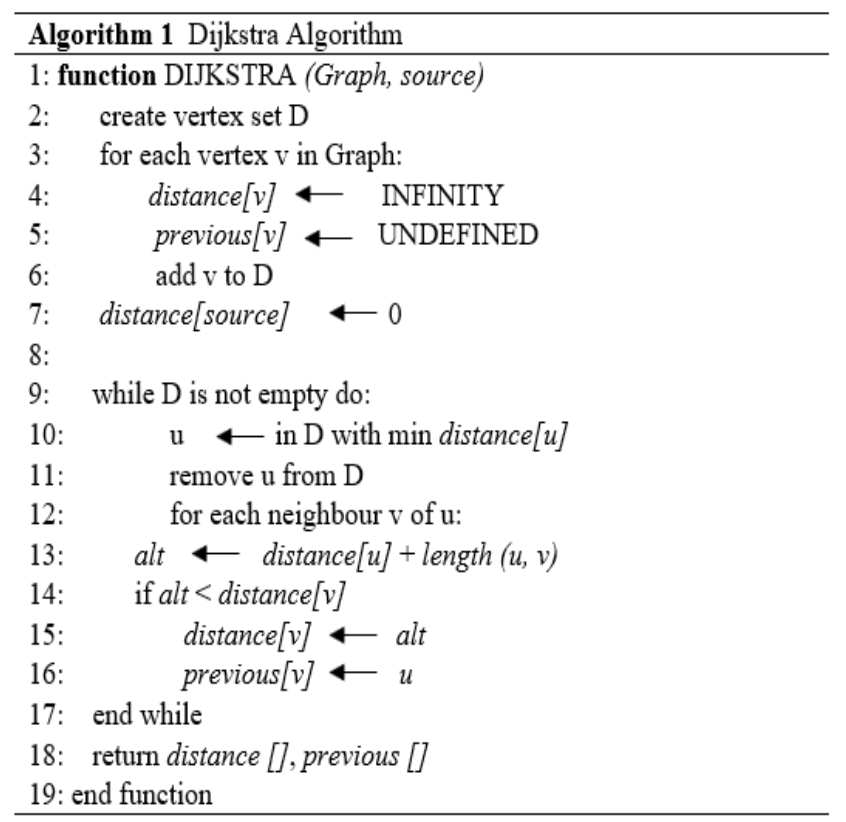
\includegraphics[width=1.0\textwidth]{images/Dijkstra_pseudoCode.PNG}
	\caption{\label{fig:Dijkstra}Dijkstra Algorithmus Pseudo-Code \cite{Abusalim2020}.}
\end{figure}

Abusalim Samah, Ibrahim Rosziati, Saringat Mohd, Jamel Sapiee und Wahab Jahari haben  diesen Pseudocode wie folgt beschrieben:
\newline
\newline
 „Beim Dijkstra-Algorithmus ist der Pfad nicht bekannt. Die Knoten werden in zwei Gruppen unterteilt: temporäre (t) und permanente (p).
\begin{itemize}
	\item  Zunächst wird die Entfernung des Quellknotens mit dem Wert Null initialisiert [distance(a) = 0], und die Entfernung der anderen Knoten wird mit dem Wert Unendlich belegt [distance(x) = infinity]. 
	\item Schritt 2: Suche nach dem Knoten x mit dem kleinsten Wert von d(x). Wenn es keine temporären Knoten gibt oder der Wert von d(x) gleich unendlich ist, wurde der Knoten x als permanent eingestuft, was bedeutet, dass sich d(x) und der übergeordnete Wert von d(x) nicht mehr ändern werden. 
	\item Schritt 3: Wenden Sie den folgenden Vergleich für jeden temporären Knoten mit der Bezeichnung vertex y an, der an x angrenzt“\footnote{Ausführliche Beschreibung von Dijkstra Pseudo Code \cite{Abusalim2020}}.
\end{itemize}


\section{Bellman-Ford-Algorithmus}
\label{Bellman-Ford-Algorithmus}
\subsection{Definition}

Vaibhavi Patel und Prof.ChitraBaggar haben benotet dass, „Der Bellman-Ford-Algorithmus verwendet Entspannung, um kürzeste Pfade auf gerichteten Graphen zu finden, die nur eine Quelle haben“\footnote{Bellman-Ford-Algorithmus Definition \cite{Vaibhavi2014}}.
\subsection{Prinzip}
Wenn es negative Gewichtsnusszyklen gibt, wird der Algorithmus sie erkennen. Eine negative Länge gibt es nicht, wenn es sich um Bereiche auf einer Karte handelt. Der Ballmann-Ford-Algorithmus ist im Allgemeinen mit dem Dijkstra-Algorithmus vergleichbar. Er entspannt alle Kanten |V| mal, wobei |V| die Menge der Scheitelpunkte ist\cite{Vaibhavi2014}.

\subsection{Bellman-Ford Pseudo-Code}\index{Bellman-Ford}
Der Bellman-Ford-Algorithmus wird wie in der Abbildung unten dargestellt ausgeführt.


 \begin{figure}[H]
	\centering
	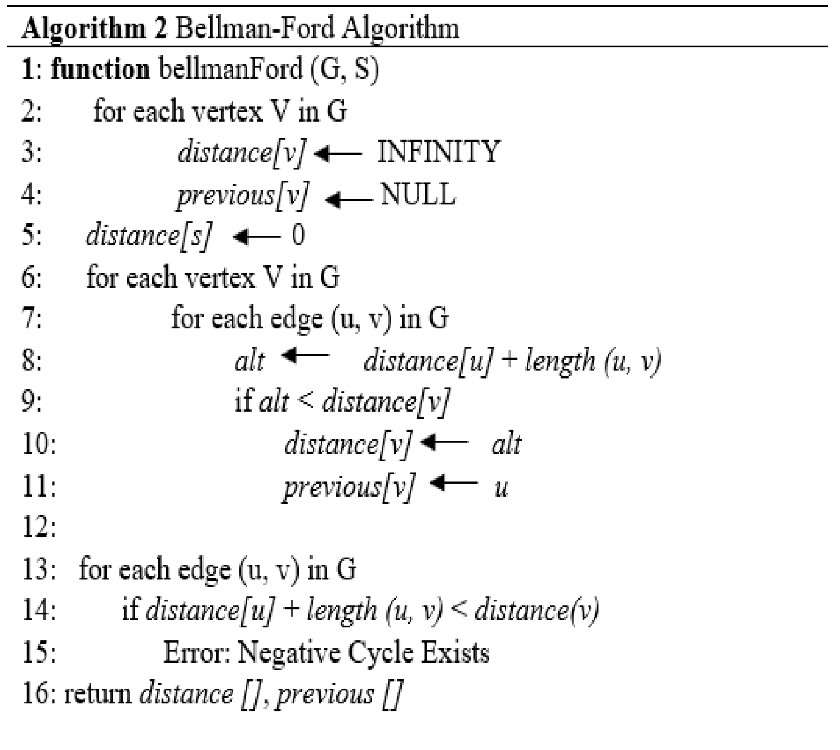
\includegraphics[width=1.0\textwidth]{images/Bellman-Ford-Algorithmus_Pseudo-Code.PNG}
	\caption{\label{fig:Bellman}Bellman-Ford Pseudo-Code\cite{Abusalim2020}.}
\end{figure}
Abusalim Samah, Ibrahim Rosziati, Saringat Mohd, Jamel Sapiee und Wahab Jahari haben sie diesen Pseudocode wie folgt beschrieben:
\newline
\newline
\begin{itemize}
	\item   „Schritt 1: Setzen Sie den Abstand des Quellknotens s auf den Wert Null (distance[s] = 0) und weisen Sie den anderen Knoten einen Abstand von INFINITY zu. 
	\item Schritt 2: entspannt jede Kante (n - 1) Mal, wenn n die Anzahl der Knoten ist. Das Entspannen einer Kante bedeutet zu prüfen ob es möglich ist, den Weg zu dem Knoten, auf den die Kante zeigt, zu verkürzen, und, wenn ja, den Weg zu den Knoten durch die gefundene Route. 
	\item Schritt 3: Prüfen, ob der Graph einen negativen Zyklus hat, mit Ausführung der N-ten Schleife“\footnote{Ausführliche Beschreibung von Bellman-Ford Pseudo Code \cite{Abusalim2020}}.
\end{itemize}







